%Chapter 1

\renewcommand{\thechapter}{1}

\chapter{Introduction}

Mobile devices pervade our daily lives. Surveys from the Pew research
center show that smartphone ownership among US adults grew from just
35\% in 2011 to 77\% in 2016~\cite{pewmobile}. With these devices
ever-present in our daily lives, it is crucial that users be able to
understand the devices' security mechanisms.

Mobile devices have access to a wide range of sensitive resources: the
user's camera, microphone, text messages, and more. Apps can use these
sensitive resources to help perform tasks and create a
contextually-aware experience. For example, an app may read the user's
text messages to eliminate spam or take a picture after some amount of
time. But the ability for apps to access these sensitive resources
leaves open the possibility of misuse.

To combat this, mobile operating systems implement security
mechanisms. iOS and Android (together comprising over 99\% of the
smartphone market~\cite{vincent_2017}) both implement a
\emph{permission} system that apps must honor. Permissions enable an
app to access private resources. Before an app uses a sensitive
resource, the app must have been granted access to the corresponding
permission (e.g., \code{CAMERA}).

All security mechanisms balance transparency with habituation. On one
hand, the system may ask users for permission every time a resource is
used by an app. This may achieve more transparency, but with the risk
that users may begin to ignore notifications~\kris{cite}. On the other
hand, the system may ask for permission only \emph{once}, but this
risks the user being unaware of certain accesses. At the time of
writing, both Android and iOS ask for permission only once for each
app.

It has recently been suggested~\cite{Nissenbaum:2004} that security
decisions are largely influenced by context. Specific to mobile
devices, there is a large amount of
work~\cite{King:2012,Balebako:2013,Fu:2014,Wijesekera:2015} to suggest
that app context deeply informs user security decisions. Indeed, in
early versions of the Android OS, permissions were authorized at the
time of app installation. Unfortunately, users rarely understood or
even read the list of permissions~\cite{Felt:2012soups}.

Context is naturally established in apps by the user's interactions
with the UI. For example, the user will likely expect that the app may
take a picture after clicking on a specific ``take photo'' icon, but
not when the phone is sitting on their desk. This motivates the notion
of \emph{interaction-based} security. I define interaction-based
security as security and privacy policies which are informed by the
user's interaction with the user interface of an application.

Thus, I end up with the following thesis:

\textit{ \indent Interaction-based security can be supported in mobile
  operating systems without any changes to the underlying
  system. Further, formal notions of security (such as information
  flow) can be naturally modified to accommodate interaction-based
  security. With advances to program understanding tools, we can aid
  auditors in quickly discovering interaction-based security
  policies.}

To substantiate this thesis, I introduce four main pieces of work that
illustrate how program analysis and understanding can be used to
support interaction-based security. The first is Redexer, a binary
rewriter for Android. Redexer allows a variety of transformations to
be performed on Android apps. For example, it allows retrofitting apps
with finer grained permissions so that users may control the
granularity of location information given to an app.

Next, I introduce interaction-based information flow policies. These
policies formally relate the information released by an app to
sequences of UI interactions made by the user. I illustrate a tool,
ClickRelease, which operates on Android apps to check that they
satisfy interaction-based policies. However, this
work~\cite{micinski:15} merely assumes that interaction-based policies
will be beneficial to users. Next, I directly study users to
understand how user interactions relate to intuitions about when
resources are used. I do this by performing both an app study and a
user study, to understand how top apps access resources and understand
how this relates to user expectations.

Last, I use a novel combination of execution logging, symbolic
execution, and abstract interpretation to design a tool which allows a
security auditor to quickly understand the different circumstances
under which permissions may be used by an app. I conclude by
commenting on how we can apply the lessons learned in this work to
enhance app security, and highlight future directions of work in this
area.

Note that within this dissertation, I focus on the Android operating
system. I speculate that the principles I propose (namely,
interaction-based security) could offer insight about other mobile
operating systems (such as iOS), but have not explored them
systematically within the context of those systems.

\section{Binary Rewriting for Enhanced Security on Android}

I begin by describing
Redexer~\cite{jsjeon:spsm12,micinski:most13}. Redexer is a tool I
(along with my colleagues) built to perform static binary rewriting on
Android apps. Binary rewriting is useful for a variety of
transformations to Android apps, and I rely upon Redexer for
subsequent chapters of this dissertation. In Chapter 3, I outline one
specific use of Redexer to replace the default Android location API
with an API that offers coarser access to the user's location.

Rewriting Dalvik bytecode is challenging because of the many subtle
invariants to which the bytecode structure must adhere. For example,
instructions include register ranges which they are allowed to
address. Redexer tackles this by giving the programmer an API that
allows inserting bytecode inside of a method without maintaining these
invariants. Redexer includes passes that clean up rewritten bytecode
to maintain these invariants, which greatly simplifies writing binary
transformations.

\section{Interaction-Based Declassification Policies}

Permissions protect the ways in which data enters apps. However, once
apps read data, permissions do not guard what apps do with that
data. \emph{Information flow}~\cite{Denning:1975} allows formally
reasoning about how sensitive data is released by applications to
(potentially untrusted) observers. One standard information-flow
property is noninterference: a public observer can learn nothing about
the private inputs to the program. In practice, information flow is
challenging to apply because many realistic applications leak
information by design (e.g., telling the user they entered the wrong
password leaks the fact that the password was not what they guessed).

There has been a large amount of
work~\cite{Sabelfeld:2009,Askarov:2007,Chong:04,Walker:00,Li:05,Sabelfeld:05}
on incorporating \emph{declassification} into noninterference. While
there is some work~\cite{O'Neill:2006,Dimitrova:12} that addresses
information flow for interactive systems, no work allows incorporating
the user interface into information flow properties.

I present \emph{interaction-based declassification} to allow
incorporating an app's user interface into information flow
policies~\cite{micinski:15}. This allows us to state policies such as
the following:

\begin{displaymath} \small
  \begin{array}{cc}
      \code{ph}!\ast \wedge (\tfuture (
      \code{sendBtn!unit} \land
      \tlast{\code{phBox}}{\code{true}})) \rhd Low \\
    \end{array}
\end{displaymath}

Here, the \code{ph!*} notation is used to represent a write of any
value on the channel \code{ph}, which is used here to represent the
phone number.  The policy can be read as follows: ``At time $i$, if
the input at time $i$ is on the \code{ph} channel, and at some
\emph{future} (indicated by the stylized $\mathcal{F}$) point $j$, the
send button is pressed (\code{sendBtn!unit}) \emph{while} the last
setting of the \code{phBox} was true, the input at time $i$ may be
declassified to security level $Low$.''

Because these policies rely on precise temporal orderings of program
states, I used \emph{symbolic execution}, a program analysis that
executes the program with symbolic variables. In a previous
collaboration I worked on SymDroid~\cite{Jeon:2012}, a symbolic
executor for Dalvik bytecode. I extended SymDroid to create
ClickRelease. ClickRelease checks these interaction-based policies by
collecting pairs of program paths and forming equations over
them. These equations encode interaction-based declassification to
guarantee that apps only leak data in accordance with the policy. I
applied ClickRelease on four synthetic apps including benign and (two)
malicious variants of those apps. ClickRelease was able to find
information flow leaks in the malicious variants and generate
counterexamples.

\section{User Interactions and Permission Use on Android}

After defining and enforcing interaction-based declassification, I ran
two studies to understand to what extent such policies match user
perceptions of security~\cite{micinski2017user}. The first measures
150 top apps to determine the interaction patterns apps used to access
permissions, and one that measures users to test how closely those
patterns align with user expectation.

I first understand the relation between an app's GUI and how it
accessed sensitive resources. My technique works by using
instrumentation to logs paths through the app as it is
executed~\cite{micinski2017}. I implemented this in a tool
called AppTracer.  AppTracer inserts instrumentation into an app that
logs its control flow. I can then run it on a device either manually
or via automated exploration and capture an execution log. Next,
AppTracer transforms this log of program behavior into an execution
graph that helps an auditor understand which GUI events caused which
permission uses. AppTracer is based on temporal sequences of events
executed by an app.

I ran AppTracer on 150 popular Android apps to classify the types of
interactive resource use in those apps. I used the graph AppTracer
produced and a human-curated codebook to assign a set of codes to each
permission use within each app. For example, in the graph below
(a subgraph of one produced by AppTracer), the app read the contacts
immediately after a button click, which is coded as a $Click$ use of
that permission.

\begin{figure}[h]
  \begin{center}
    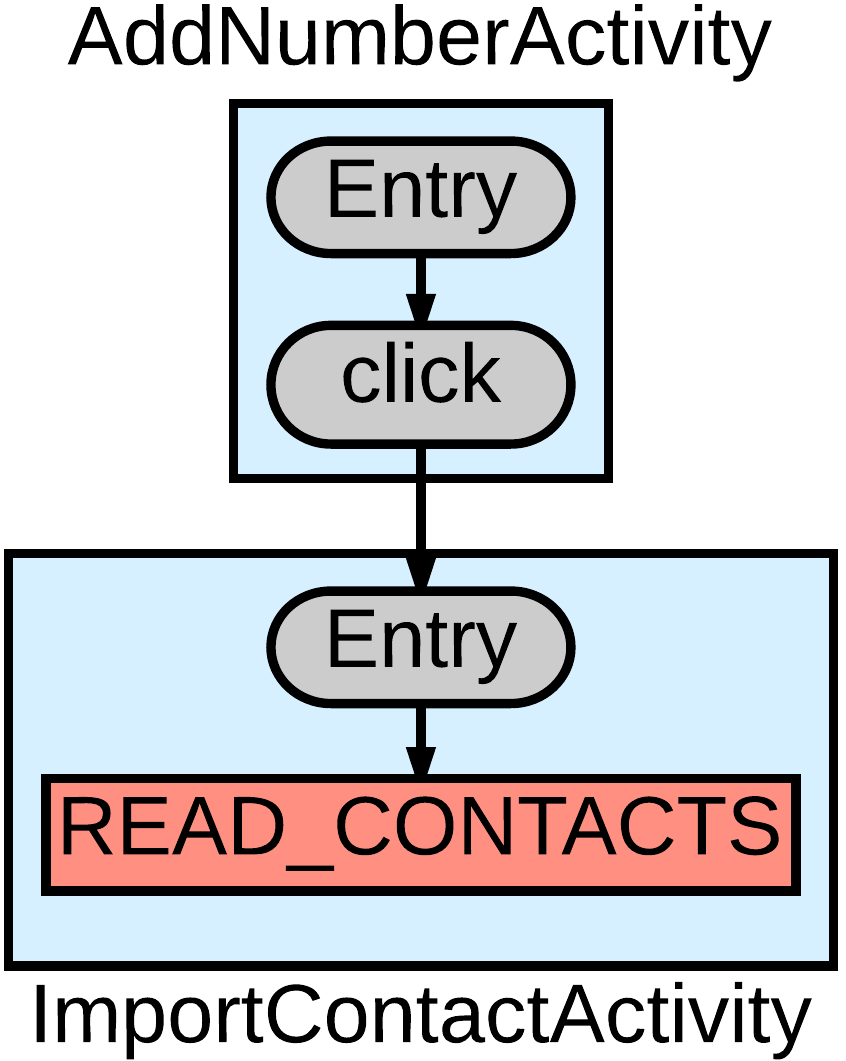
\includegraphics[width=2in]{click.png}
  \end{center}
\end{figure}

Next, I conducted a user study. This study evaluated when users
expected permission use to occur with respect to the app's GUI. It is
comprised of a walkthrough of an app interspersed with questions about
what resources the user expects will be used.  For example, in one
scenario the user first sees an app's home screen, then presses the
``voice order coffee'' button. To mirror the current Android
permissions system, they are then prompted to allow access to the
microphone --- in other scenarios this dialog occurs at the beginning
of the app or not at all to measure the effect of timing on user
expectation. After seeing the dialog, the user is asked a series of
Likert-style questions assessing their expectation the microphone will
be used at that point in the app. The user is then shown another
interaction with the app, in this case going back to the phone's home
screen. They are again asked expectation questions to understand how
their perceptions of permission use changes as context changes.

Combining the results of the two studies, I discovered that apps
mostly matched user expectations, but noted some shortcomings with the
permission system. Users seemed to expect the most invasive
permissions (e.g., camera and microphone) to be used only after a
click. Our app study confirmed this is almost exclusively the case. We
recommend that this be made mandatory with rare exceptions, since uses
of these resources not clearly associated with a relevant click are
unexpected by users. Even when users understand resources will be
accessed after these clicks, Android still asks users for explicit
permission via a dialog screen. This implies Android is being too
invasive, and that these interactions alone are sufficient to
authorize the permission use. Also, we found that when users were
prompted for permission immediately after a click, they assumed that
that resource was used \emph{only} after that interaction. For
example, if an app waits until a map screen to ask users for location,
users will be much less likely to expect the location to be used later
in the app (perhaps, e.g., while the app is off the screen). We
observed infrequent but occasional uses of this in our app study.

\section{Permission-Use Provenance in Android Using Sparse Dynamic Analysis}

AppTracer helps understand why apps use permissions, but it worked
based on traces of app events. Because of this, AppTracer would
associate permission uses with UI elements that were temporally close
to permission uses. This worked well for many cases we looked at,
where permissions were used immediately after clicking on a button, or
after the user navigated to a new screen. However, it was more
challenging to understand background uses of permissions. Our user
study suggested that these background uses may be tricky for users to
understand, so I decided to pursue tools that would help understand
these permission uses. 

In Chapter 6 I introduce Hogarth, a system which uses a combination of
app logging, symbolic execution, and abstract interpretation to
explain permission uses within apps. The goal of Hogarth is to present
a path through an app that elicits a permission use. Android apps are
callback-oriented, which makes it challenging to define what it means
to take a path through an app. Hogarth tackles this problem by
observing that callbacks may register other callbacks, and building a
graph of callbacks which influence each other. It then presents a
graph of app behavior, where nodes in this graph are callbacks (some
containing permission uses) and edges connect callbacks when one
callback registers another.

Connecting callbacks allows an auditor to understand roughly where a
permission is used within an app's source code. However, it does not
allow a user to understand why that permission is used. To explain
this, Hogarth also reconstructs a \emph{path condition} that holds
along every path to the permission use within the body of logs. It
does this by borrowing techniques from abstract interpretation to
collecting the constraints that held on every path reaching a
permission, and using a constraint solver to produce a minimal formula
that reaches the points at which permissions are used. I applied
Hogarth to five moderately-sized Android apps from the F-Droid app
store and the contagio malware dataset. I found that---while Hogarth
is still a prototype---it was effectively able to recover path
conditions that were found by otherwise time-consuming
reverse-engineering efforts.


